\documentclass[a4paper,12pt]{article}

% Pakete für grundlegende Funktionalitäten
\usepackage[utf8]{inputenc}
\usepackage[T1]{fontenc}

% Pakete für Code, Tabellen und Hyperlinks
\usepackage[utf8]{inputenc}
\usepackage{listings}
\usepackage{xcolor}
\usepackage[hidelinks]{hyperref} % Entfernt die roten Rahmen um Hyperlinks
\usepackage{graphicx}



\usepackage{booktabs}


\lstset{
    basicstyle=\ttfamily\small,    % Monospace-Schriftart und kleine Schrift
    breaklines=true,               % Automatischer Zeilenumbruch
    frame=single,                  % Rahmen um den Codeblock
    backgroundcolor=\color{gray!10}, % Grauer Hintergrund
    xleftmargin=1em,               % Leichter linker Rand
    xrightmargin=1em,              % Leichter rechter Rand
    columns=flexible,              % Korrekte Ausrichtung der Zeichen
    keywordstyle=\normalfont,      % Keine Hervorhebung von Keywords
    stringstyle=\normalfont,       % Keine Hervorhebung von Strings
    captionpos=b,                  % Beschriftung unten
    showstringspaces=false,        % Keine Leerzeichensymbole
    commentstyle=\normalfont,      % Kommentare normal darstellen
    numbers=none                   % Keine Zeilennummern
}




\documentclass[a4paper,12pt]{article}
\usepackage[utf8]{inputenc}
\usepackage[T1]{fontenc}
\usepackage{graphicx}
\usepackage{geometry}
\usepackage{setspace}
\usepackage{lmodern}

% Seitenränder
\geometry{top=3cm, bottom=3cm, left=3cm, right=3cm}

% Schriftart und Zeilenabstand
\renewcommand{\baselinestretch}{1.5}

% Begin des Dokuments
\begin{document}

% Keine Seitenzahlen auf dem Deckblatt
\pagenumbering{gobble}

% Logo der Fachhochschule (optional)
\begin{figure}[t]
    \centering
    
\includegraphics[width=0.25\textwidth]{FHGR.jpeg} % Logo-Pfad anpassen
\end{figure}

\vspace{2cm}

% Titel der Arbeit
\begin{center}
    {\Huge \textbf{Raspberry Pi als Cloud-Lösung und Entwicklungsplattform}} \\[1.0em]
    {\Large \textit{Von der Einrichtung des Systems bis zur Datenanalyse in der Cloud}} \\
\end{center}

\vspace{3cm}

% Persönliche und akademische Informationen
\begin{center}
    \textbf{Erstellt von:} \\[0.5em]
    {\Large Frédéric C. Kurbel} \\[1.5em]
    
    Studiengang: \textbf{Computational and Data Science} \\[1.5em]
    
    Modul: \textbf{Computer Science} \\[0.5em]
    Professor: \textbf{Ana Petrus} \\
\end{center}

\vspace{3cm}

% Abgabedatum
\begin{center}
    \textbf{Abgabedatum: 14.12.2024} \\
\end{center}

\vfill

% Fußzeile (falls gewünscht)
\begin{center}
    \rule{0.8\textwidth}{0.5pt} \\[0.5em]
    \textbf{Fachhochschule Graubünden}
\end{center}

% Inhaltsverzeichnis
\renewcommand{\contentsname}{Inhaltsverzeichnis}

\tableofcontents
\newpage

\section{Einleitung}

\subsection{Überblick zum Projekt}
Diese Dokumentation beschreibt den Prozess der Einrichtung eines Raspberry Pi als Cloud-Server, das Einrichten einer SQL-Datenbank und die Ausführung von Python-Skripten innerhalb der Cloud. Der Fokus liegt auf der Installation und Konfiguration der Hardware und Software sowie auf einem Beispiel zur Datenanalyse. Das Projekt bietet eine Grundlage für weiterführende Arbeiten im Bereich Data Science und Automatisierung.

\subsection{Der Raspberry Pi}
Der Raspberry Pi ist ein kostengünstiger und vielseitiger Einplatinencomputer, der häufig für Projekte in den Bereichen Cloud-Computing, Automatisierung und IoT verwendet wird. In diesem Projekt wurde ein Raspberry Pi 4 als Grundlage für die Implementierung einer Cloud-Lösung und die Ausführung von Python-Skripten eingesetzt.

\begin{figure}[h!]
    \centering % Zentrierte Ausrichtung für professionelleres Layout
    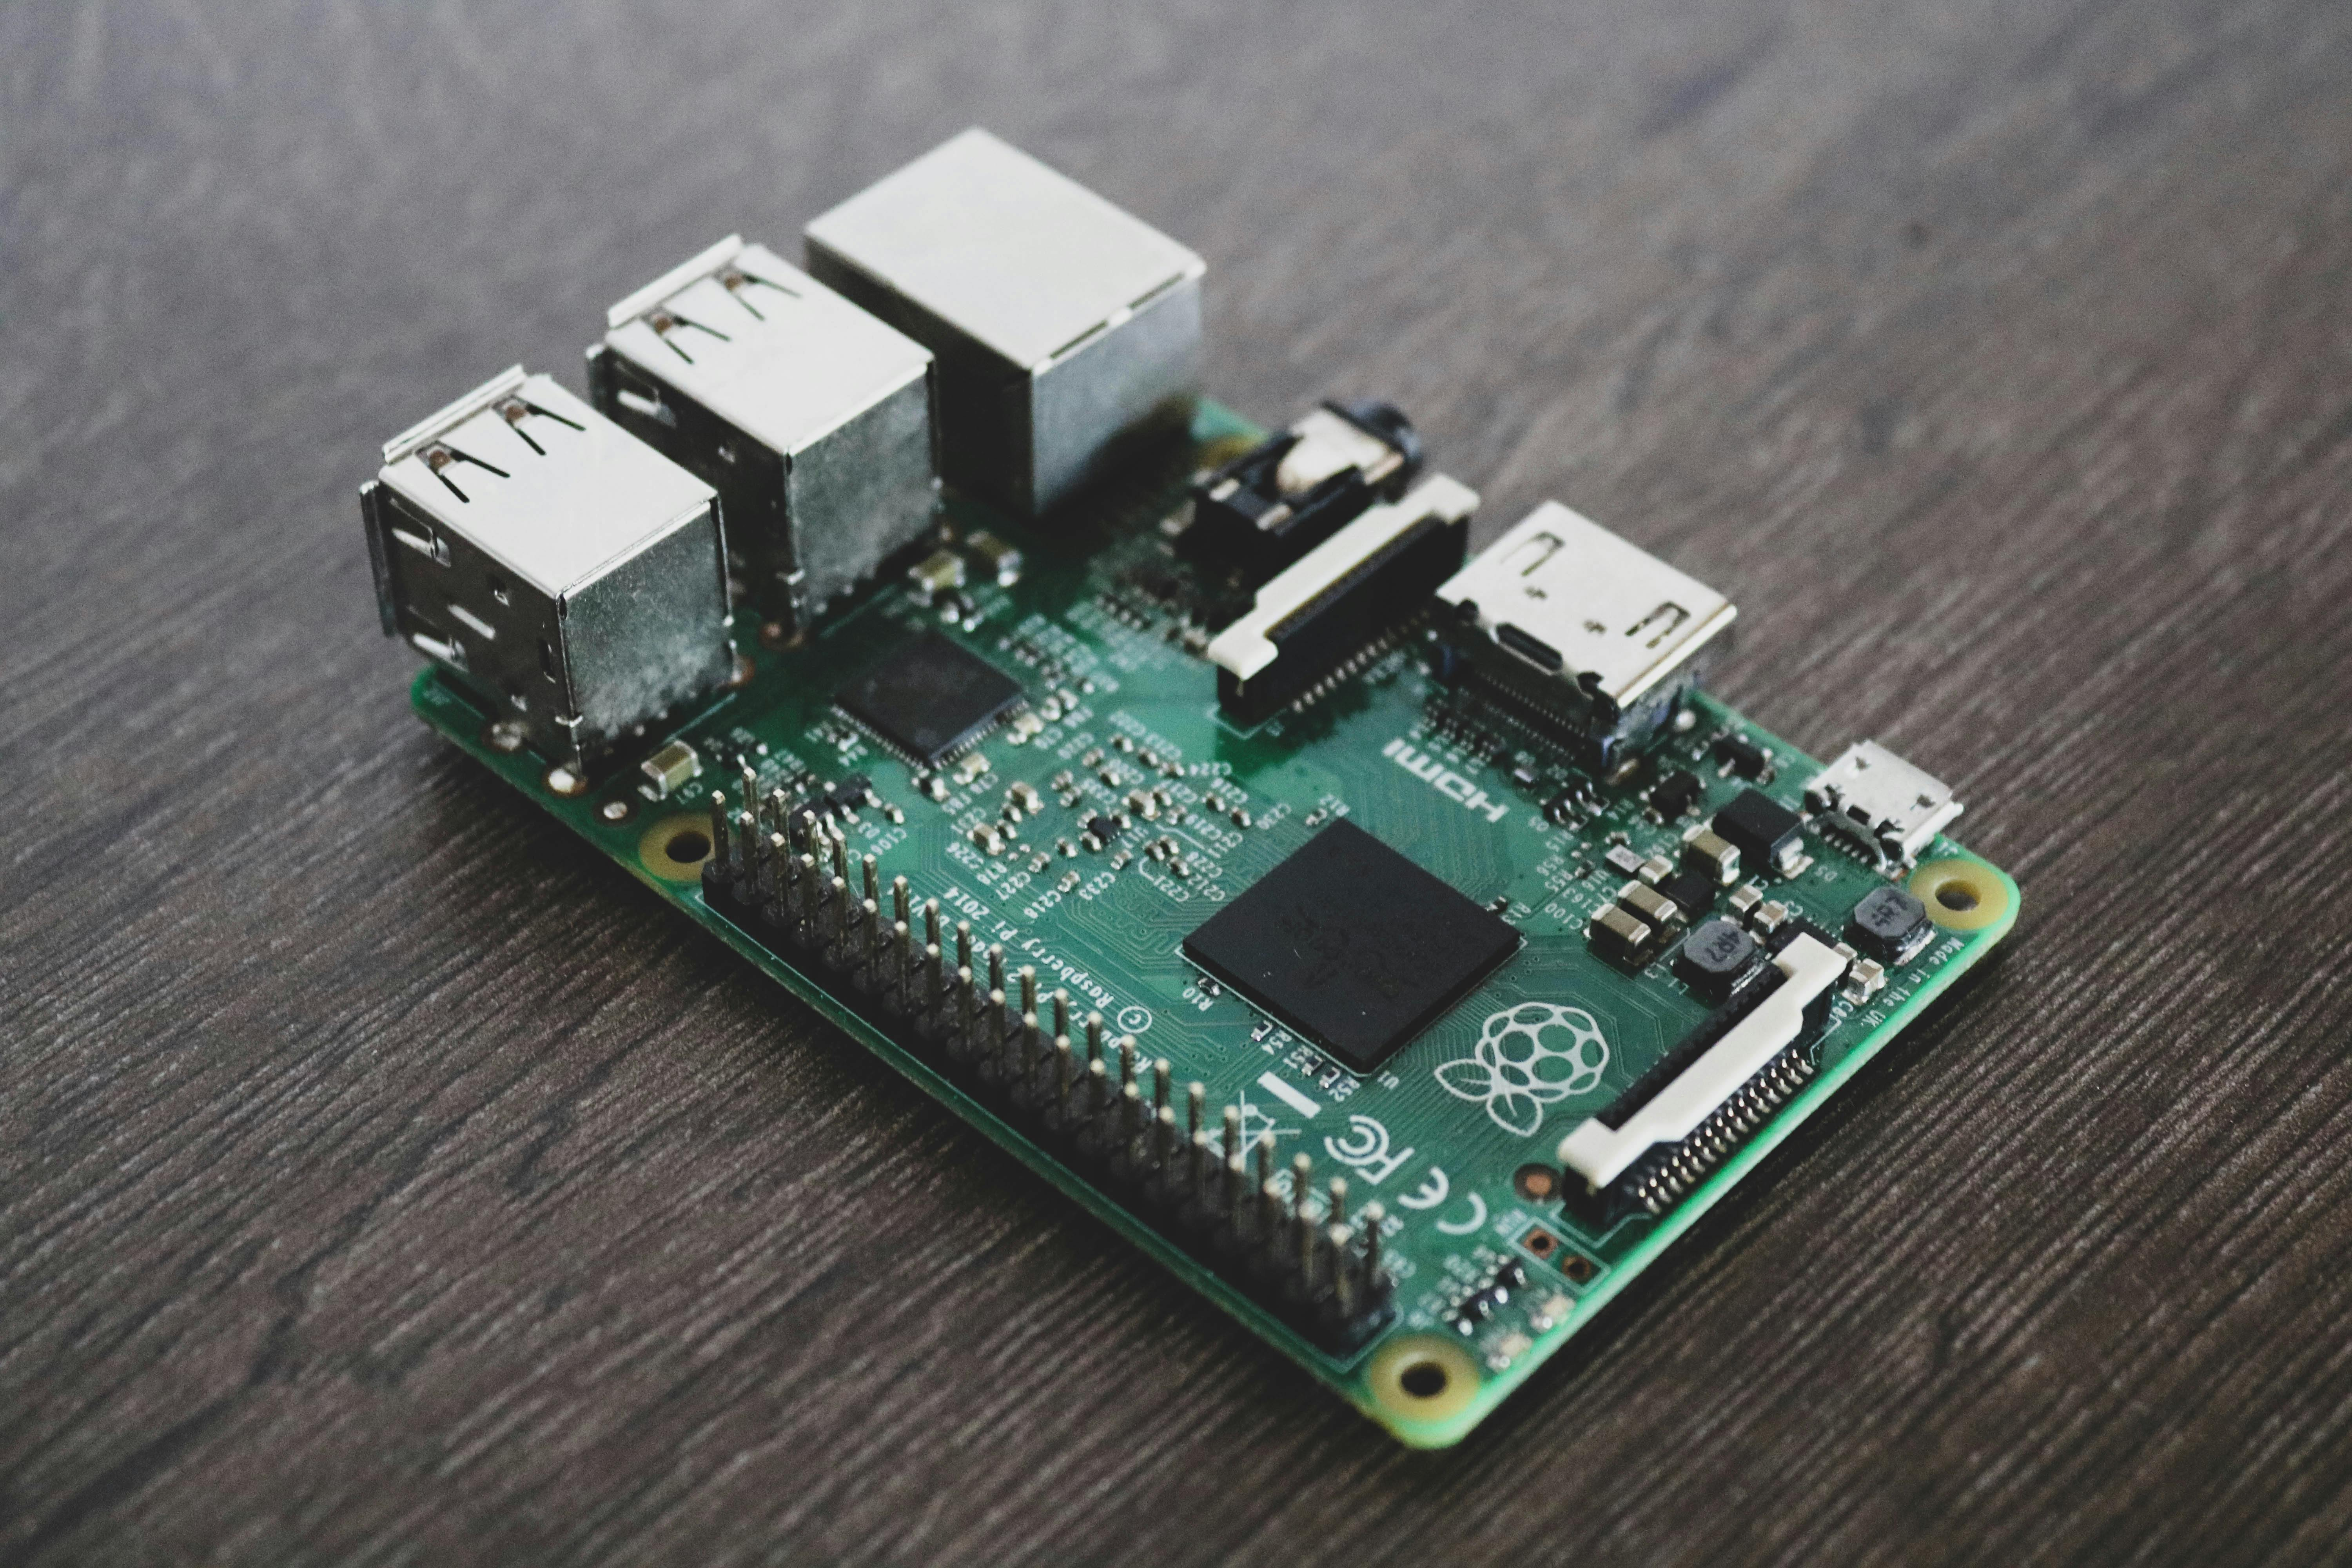
\includegraphics[width=0.7\textwidth]{pexels-alessandro-oliverio-611273-1472443.jpg}
    \caption{Ein Raspberry Pi 4, wie er in diesem Projekt verwendet wurde.}
    \label{fig:raspberry_pi}
\end{figure}

\noindent
Im Folgenden wird detailliert beschrieben, wie der Raspberry Pi eingerichtet und konfiguriert wurde, um als Cloud-Server mit SQL-Unterstützung und Jupyter Notebook zu dienen.

\subsection{Projektressourcen}
Um den Quellcode sowie weiterführende Informationen zu diesem Projekt abzurufen, besuchen Sie das zugehörige GitHub-Repository:  
\url{https://github.com/Fredeys/raspberry-pi_cloud_dev}.


\section{Methodik}
Die Methodik gliedert sich in drei Hauptbereiche:
\begin{enumerate}
    \item Einrichtung des Raspberry Pi (Hardware und Betriebssystem).
    \item Konfiguration eines Cloud-Servers (Webserver und Datenbank).
    \item Anwendung von Python-Skripten in der Cloud.
\end{enumerate}

\section{Raspberry Pi – Einrichtung}
\subsection{Installation des Betriebssystems}
\begin{enumerate}
    \item Setze die SD-Karte in einen PC oder Laptop ein und lade den \textit{Raspberry Pi Imager} von \url{https://www.raspberrypi.com/software/} herunter.
    \item Wähle das Betriebssystem \textit{Raspberry Pi OS (64-BIT)}.
    \item Konfiguriere Benutzername, Passwort, Landeseinstellungen und WLAN-Verbindung.
    \item Installiere das Betriebssystem auf der SD-Karte und überprüfe die Installation.
    \item Entnehme die SD-Karte und setze sie in den Raspberry Pi ein.
\end{enumerate}

\subsection{Netzwerkverbindung und SSH-Zugriff}
\begin{enumerate}
    \item Lade \textit{Angry IP Scanner} von \url{https://angryip.org} herunter. Alternativ können auch andere Lösungen verwendet werden, die IP-Adressen von Geräten im Netzwerk auffinden.
    \item Identifiziere die IP-Adresse des Raspberry Pi im lokalen Netzwerk.
    \item Verbinde dich über SSH mit dem Raspberry Pi. Verwende dafür den zuvor festgelegten Benutzernamen und die IP-Adresse:
\begin{lstlisting}[language=bash]
ssh Benutzername@IP-Adresse 
\end{lstlisting}
    \item Nach dem Ausführen des Befehls erscheint folgende Meldung, wenn es die erste Verbindung zu diesem Host ist:
\begin{lstlisting}[language=bash]
The authenticity of host 'IP-Adress' (IP-Adress) cant be established.
ED25519 key fingerprint is SHA256:QLdRk69v5I0ZAut3CVMmCAdwuqzXpGSymdHJB/FWars.
Are you sure you want to continue connecting (yes/no/[fingerprint])?
\end{lstlisting}
    \item Bestätige die Verbindung durch Eingabe von \texttt{yes}. Dadurch wird die IP-Adresse des Raspberry Pi zur Liste der bekannten Hosts hinzugefügt:
\begin{lstlisting}[language=bash]
Warning: Permanently added 192.168.1.51 (ED25519) to the list of known hosts.
\end{lstlisting}
    \item Logge dich mit dem zuvor festgelegten Passwort ein. Beachte, dass das Passwort aus Sicherheitsgründen nicht im Terminal angezeigt wird.
    \item Konfiguriere den Raspberry Pi mit folgendem Befehl:
\begin{lstlisting}[language=bash]
sudo raspi-config
\end{lstlisting}
    Durch den Befehl wird Zugriff zur graphischen Benutzeroberfläche erlangt, und die Einstellungen können angepasst werden:
    \begin{itemize}
        \item Wähle \textit{Interface Options}.
        \item Wähle \textit{VNC Enable/disable graphical remote desktop access} und bestätige mit \texttt{<Yes>}. Die darauf folgende Meldung \textit{The VNC Server is enabled} kann mit \texttt{<Ok>} bestätigt werden.
        \item Wähle \texttt{<Finish>}, um wieder in das Raspberry Terminal zu gelangen.
    \end{itemize}
\end{enumerate}

\section{VNC-Viewer Einrichtung}
\subsection{Download und Installation des VNC-Viewers}
Der VNC-Viewer kann über den folgenden Link heruntergeladen werden:  
\url{https://www.realvnc.com/de/connect/download/viewer/macos/?lai_vid=WKMJdXxyOHBkz&lai_sr=0-4&lai_sl=l&lai_p=1}

\subsection{Verbindung zum Raspberry Pi herstellen}
Nach dem Öffnen der Applikation wird eine neue Verbindung angelegt:
\begin{itemize}
    \item Für den Input \textit{VNC-Server} wird die zuvor ermittelte IP-Adresse des Raspberry Pi verwendet.
    \item Ein Name für die Verbindung wird vergeben, um das Projekt leichter identifizieren zu können.
\end{itemize}

\subsection{Authentifizierung und Zugriff}
Um die Verbindung zum Raspberry Pi herzustellen, sind folgende Schritte erforderlich:

\begin{enumerate}
    \item Beim ersten Verbindungsaufbau erscheint die folgende Meldung:
    \begin{lstlisting}[language=bash]
Identity Check - VNC Viewer has no record of connecting to this VNC Server,so its identity cannot be checked.
    \end{lstlisting}
    Diese Warnung weist darauf hin, dass die Verbindung zum VNC-Server nicht überprüft werden kann. Bestätige die Meldung durch Klicken auf \textit{Continue}.
  
    \item Nach der Bestätigung fordert der VNC-Viewer eine Authentifizierung an. Gib hierfür die folgenden Zugangsdaten ein:
    \begin{itemize}
        \item \textbf{Benutzername}: Der Benutzername, der während der Einrichtung des Raspberry Pi festgelegt wurde.
        \item \textbf{Passwort}: Das ebenfalls während der Einrichtung festgelegte Passwort.
    \end{itemize}
    
    \item Nach erfolgreicher Authentifizierung erhältst du Zugriff auf die graphische Oberfläche des Raspberry Pi.
\end{enumerate}

\subsection{Graphischer Zugriff auf den Raspberry Pi}
Nach der erfolgreichen Authentifizierung kann der VNC-Viewer auf die graphische Oberfläche des Raspberry Pi zugreifen. Um den VNC-Server zu starten, verwende den folgenden Befehl im Raspberry Terminal:
\begin{lstlisting}[language=bash]
vncserver-x11
\end{lstlisting}

\subsection{Zusätzlicher Hinweise}
Falls ein VNC-Account erstellt und mit dem VNC-Viewer verknüpft wird, ist der Zugriff auf den Raspberry Pi auch ortsunabhängig möglich.

\section{Cloud-Setup}
\subsection{Installation des Webservers}
Zur Bereitstellung der Cloud wird der \textit{Apache}-Webserver verwendet. Die Installation erfolgt mit folgenden Befehlen:
\begin{lstlisting}[language=bash]
sudo apt update
sudo apt install apache2 -y
sudo apt install php php-gd php-curl php-zip php-xml php-mysql -y
\end{lstlisting}

\subsection{Einrichtung der Datenbank}
\textit{MariaDB} wird als Datenbank-Management-System installiert und konfiguriert. Die Installation erfolgt mit folgendem Befehl:
\begin{lstlisting}[language=bash]
sudo apt install mariadb-server -y
sudo mysql_secure_installation
\end{lstlisting}

\noindent
Nach der Installation erfolgt die Konfiguration. Es werden folgende Schritte durchgeführt:

\begin{enumerate}
    \item Führe den Befehl \texttt{sudo mysql\_secure\_installation} aus und beantworte die folgenden Eingabeaufforderungen:
    \begin{itemize}
        \item \textbf{Enter current password for root}: Bestätige mit der \texttt{Enter}-Taste (kein Passwort erforderlich).
        \item \textbf{Switch to unix\_socket\_authentication? [Y/n]}: Antworte mit \texttt{n}, um diese Option abzulehnen.
        \item \textbf{Change the root password? [Y/n]}: Antworte mit \texttt{n}, um kein neues Passwort zu setzen.
        \item \textbf{Remove anonymous users? [Y/n]}: Antworte mit \texttt{Y}, um anonyme Benutzer zu entfernen.
        \item \textbf{Disallow root login remotely? [Y/n]}: Antworte mit \texttt{Y}, um Root-Logins über das Netzwerk zu verbieten.
        \item \textbf{Remove test database and access to it? [Y/n]}: Antworte mit \texttt{Y}, um die Test-Datenbank zu löschen.
        \item \textbf{Reload privilege tables now? [Y/n]}: Antworte mit \texttt{Y}, um die Privilegientabellen neu zu laden.
    \end{itemize}
    
    \item Nach Abschluss dieser Schritte melde dich bei MariaDB an:
\begin{lstlisting}[language=bash]
sudo mysql -u root -p
\end{lstlisting}
    Wenn du zur Eingabe eines Passworts aufgefordert wirst (\textit{Enter password:}), kannst du entweder ein neues Passwort setzen oder mit der \texttt{Enter}-Taste fortfahren.
    
    \item Nachdem du Zugriff auf MariaDB erhalten hast, lege eine neue Datenbank an und konfiguriere die Benutzerrechte:
\begin{lstlisting}[language=bash]
CREATE DATABASE nextcloud;
GRANT ALL ON nextcloud.* TO 'nextclouduser'@'localhost' IDENTIFIED BY 'deinPasswort';
FLUSH PRIVILEGES;
EXIT;
\end{lstlisting}
\end{enumerate}

\noindent
Durch diese Schritte ist die Datenbank erfolgreich eingerichtet und bereit für die Verwendung durch Nextcloud.

\subsection{Installation von Nextcloud}
Die Installation und Konfiguration von Nextcloud erfolgt in mehreren Schritten. Alle verfügbaren Versionen können auf der offiziellen Webseite eingesehen werden:  
\url{https://download.nextcloud.com/server/releases/}

\subsubsection{Installation der Software}
Führe die folgenden Befehle im Raspberry Terminal aus, um die Software herunterzuladen und zu entpacken:
\begin{lstlisting}[language=bash]
wget https://download.nextcloud.com/server/releases/nextcloud-28.0.0.tar.bz2
tar -xvf nextcloud-28.0.0.tar.bz2
sudo mv nextcloud /var/www/html/
sudo chown -R www-data:www-data /var/www/html/nextcloud
\end{lstlisting}

\subsubsection{Konfiguration des Apache-Webservers}
Nach der Installation von Nextcloud muss der Apache-Webserver konfiguriert werden. Öffne die Konfigurationsdatei mit folgendem Befehl:
\begin{lstlisting}[language=bash]
sudo nano /etc/apache2/sites-available/nextcloud.conf
\end{lstlisting}
Füge den folgenden Inhalt in die Datei ein, speichere die Änderungen und beende den Editor:
\begin{lstlisting}[language=html]
<VirtualHost *:80>
    ServerAdmin webmaster@localhost
    DocumentRoot /var/www/html/nextcloud

    <Directory /var/www/html/nextcloud/>
        Require all granted
        AllowOverride All
        Options FollowSymLinks MultiViews

        <IfModule mod_dav.c>
            Dav off
        </IfModule>
    </Directory>

    ErrorLog ${APACHE_LOG_DIR}/error.log
    CustomLog ${APACHE_LOG_DIR}/access.log combined
</VirtualHost>
\end{lstlisting}

\noindent
Aktiviere die neue Konfiguration und die benötigten Apache-Module, und starte den Apache-Webserver neu:
\begin{lstlisting}[language=bash]
sudo a2ensite nextcloud
sudo a2enmod rewrite headers env dir mime
sudo systemctl restart apache2
\end{lstlisting}

\subsubsection{Zugriff auf Nextcloud über den Browser}
Nach der erfolgreichen Konfiguration kannst du über einen Webbrowser auf Nextcloud zugreifen. Gib dazu folgende URL ein, wobei \texttt{IP-Adresse} durch die IP deines Raspberry Pi ersetzt wird:
\begin{lstlisting}[language=]
http://IP-Adresse/nextcloud
\end{lstlisting}

\noindent
Im Browser erscheint die Installationsseite von Nextcloud. Gib folgende Informationen ein:
\begin{itemize}
    \item \textbf{Benutzername und Passwort}: Lege einen neuen Administrator-Benutzer an.
    \item \textbf{Datenbank-Konfiguration}:
    \begin{itemize}
        \item Datenbank-Benutzer: \texttt{nextclouduser}
        \item Datenbank-Name: \texttt{nextcloud}
        \item Passwort: Das während der Einrichtung festgelegte Passwort.
    \end{itemize}
\end{itemize}

\noindent
Bestätige die Installation. Nach Abschluss wirst du auf die Hauptseite weitergeleitet, auf der verschiedene empfohlene Apps zur Installation angezeigt werden. Installiere die vorgeschlagenen Apps, um die Funktionalität von Nextcloud zu erweitern.

\subsubsection{Hinweis}
Nach der Installation steht Nextcloud zur Verfügung und kann für Dateifreigabe, Synchronisation und andere Cloud-Dienste verwendet werden.

\section{Python-Skripte in der Cloud}
\subsection{Einrichtung von Jupyter Notebook}
Die Installation und Konfiguration von Jupyter Notebook erfolgt in mehreren Schritten:

\subsubsection{Installation von Jupyter Notebook}
Führe die folgenden Befehle aus, um Jupyter Notebook zu installieren:
\begin{lstlisting}[language=bash]
sudo apt update
sudo apt install python3-pip -y
pip3 install notebook
\end{lstlisting}

\subsubsection{Konfiguration von Jupyter Notebook}
Generiere die Konfigurationsdatei für Jupyter Notebook:
\begin{lstlisting}[language=bash]
jupyter notebook --generate-config
\end{lstlisting}

\noindent
Die Konfigurationsdatei wird unter dem Pfad \texttt{\textasciitilde/.jupyter/jupyter\_notebook\_config.py} erstellt. Öffne sie mit folgendem Befehl:
\begin{lstlisting}[language=bash]
nano ~/.jupyter/jupyter_notebook_config.py
\end{lstlisting}

\noindent
Füge den folgenden Code in die Datei ein, speichere die Änderungen und kehre zum Terminal zurück:
\begin{lstlisting}[language=Python]
c.NotebookApp.port = 8889
c.NotebookApp.ip = '0.0.0.0'
c.NotebookApp.open_browser = False
\end{lstlisting}

\subsubsection{Starten von Jupyter Notebook}
Starte Jupyter Notebook mit folgendem Befehl:
\begin{lstlisting}[language=bash]
jupyter notebook
\end{lstlisting}

\noindent
Hinweis: Das Terminal gibt einen Link aus, der in den Browser eingefügt werden muss, da sich das Notebook nicht automatisch öffnet.

\subsubsection{Titanic-Dataset in der Cloud speichern und verarbeiten}
Installiere das Python-Paket \texttt{seaborn} und überprüfe die Installation:
\begin{lstlisting}[language=bash]
sudo apt update
sudo apt install python3-seaborn -y
python3 -c "import seaborn as sns; print('Seaborn installiert')"
\end{lstlisting}

Speichere das Titanic-Dataset als CSV-Datei:
\begin{enumerate}
    \item Erstelle ein Python-Skript mit folgendem Inhalt:
\begin{lstlisting}[language=Python]
import seaborn as sns
import pandas as pd

# Titanic-Dataset laden
titanic = sns.load_dataset('titanic')

# Dataset als CSV speichern
titanic.to_csv('/home/pi/titanic.csv', index=False)
print("Titanic-Dataset wurde als 'titanic.csv' gespeichert.")
\end{lstlisting}

    \item Speichere das Skript als \texttt{save\_titanic.py} und führe es aus:
\begin{lstlisting}[language=bash]
python save_titanic.py
\end{lstlisting}

    \item Verschiebe die erzeugte CSV-Datei in das Nextcloud-Verzeichnis:
\begin{lstlisting}[language=bash]
sudo mv /home/pi/titanic.csv /var/www/html/nextcloud/
\end{lstlisting}

    \item Setze die Zugriffsrechte für die Datei:
\begin{lstlisting}[language=bash]
sudo chown www-data:www-data /var/www/html/nextcloud/titanic.csv
sudo chmod 644 /var/www/html/nextcloud/titanic.csv
\end{lstlisting}
\end{enumerate}

\subsubsection{Titanic-Dataset in Jupyter Notebook analysieren}
Öffne Jupyter Notebook mit dem folgenden Befehl:
\begin{lstlisting}[language=bash]
jupyter notebook --port=8889 --no-browser
\end{lstlisting}

\noindent
Erstelle ein neues Notebook und führe den folgenden Python-Code aus, um das Titanic-Dataset zu laden und die ersten Zeilen auszugeben:
\begin{lstlisting}[language=Python]
import pandas as pd

# Titanic-Dataset laden
df = pd.read_csv('/var/www/html/nextcloud/titanic.csv')
print(df.head())
\end{lstlisting}

\subsubsection{Erwarteter Output}
Die Ausgabe des Titanic-Datasets wird in drei Teilen dargestellt, um die Übersichtlichkeit zu erhöhen:

\begin{lstlisting}
   survived  pclass     sex   age  sibsp  parch  
0         0       3    male  22.0      1      0  
1         1       1  female  38.0      1      0  
2         1       3  female  26.0      0      0  
3         1       1  female  35.0      1      0  
4         0       3    male  35.0      0      0  
\end{lstlisting}

\begin{lstlisting}
     fare embarked  class     who  adult_male  
0   7.2500        S  Third     man        True  
1  71.2833        C  First   woman       False  
2   7.9250        S  Third   woman       False  
3  53.1000        S  First   woman       False  
4   8.0500        S  Third     man        True  
\end{lstlisting}

\begin{lstlisting}
     deck  embark_town      alive  alone  
0     NaN  Southampton        no  False  
1       C    Cherbourg       yes  False  
2     NaN  Southampton       yes   True  
3       C  Southampton       yes  False  
4     NaN  Southampton        no   True  
\end{lstlisting}

\noindent
Durch diese Schritte wird das Titanic-Dataset erfolgreich in der Cloud gespeichert und mit Jupyter Notebook analysiert.


\section{Ergebnisse}
Durch die beschriebenen Schritte wurde eine voll funktionsfähige Cloud auf dem Raspberry Pi eingerichtet. Python-Skripte wie Datenanalysen können in dieser Umgebung effizient ausgeführt werden. Zudem wurde eine Datenbank eingerichtet, die bislang jedoch nicht weiter verwendet wurde und für zukünftige Erweiterungen bereitsteht.

\section{Diskussion und Ausblick}
Dieses Projekt zeigt die Vielseitigkeit eines Raspberry Pi als kostengünstige und flexible Cloud-Lösung. Zukünftige Arbeiten könnten Sicherheitsaspekte wie SSL-Zertifikate oder Firewall-Konfigurationen integrieren, um die Cloud noch sicherer zu gestalten.

\section{Fazit}
Die Einrichtung eines Raspberry Pi für Cloud-Computing und Datenanalysen bietet eine exzellente Grundlage für weiterführende Projekte im Bereich Data Science und Automatisierung.

\newpage
\section{Quellen}
\begin{enumerate}
    \item Raspberry Pi Foundation. \textit{Raspberry Pi Imager}. Zugriff unter: \url{https://www.raspberrypi.com/software/}
    \item RealVNC. \textit{VNC Viewer Download}. Zugriff unter: \url{https://www.realvnc.com/connect/download/viewer/}
    \item Nextcloud. \textit{Nextcloud Releases}. Zugriff unter: \url{https://download.nextcloud.com/server/releases/}
    \item Debian. \textit{MariaDB Secure Installation Guide}. Zugriff unter: \url{https://mariadb.com/kb/en/mysql_secure_installation/}
    \item Seaborn Library. \textit{Load Titanic Dataset}. Zugriff unter: \url{https://seaborn.pydata.org/generated/seaborn.load_dataset.html}
    \item Raspberry Pi Beginner Tutorial. Zugriff unter: \url{https://www.youtube.com/watch?v=6vJeDlffCAQ}
    \item Nextcloud Installation Tutorial. Zugriff unter: \url{https://www.youtube.com/watch?v=QUl5ID4YKfw}
    \item Foto von Alessandro Oliverio von Pexels: \url{https://www.pexels.com/de-de/foto/silber-und-grun-leiterplatte-1472443/}
\end{enumerate}

\end{document}
